\chapter{Design}
\textbf{Versionshistorik}
\begin{longtabu} to \linewidth{@{}l l l X[j]@{}}
    Version &    Dato &    Ansvarlig &    Beskrivelse\\[-1ex]
    \midrule
    1.0		&	20-10-2015 &	 Alle	& Første udkast til domænemodel, BDD, IBD og sekvensdiagrammer	\\[-1ex]
    1.1		&	21-10-2015	&	Alle	& Små ændringer i BDD og IBD efter møde med vejleder \\[-1ex]
    1.2		&	27-10-2015	&	Alle	& Ændring af BDD og IBD efter møde med Kim; blokkene filter og forstærker er blevet lagt sammen under blokken Signalbehandling\\[-1ex]
    1.3  	&	02-11-2015	&	Alle	& Begyndte at oprette Design-dokumentet. Udkast til klassediagrammer for UC \\[-1ex]
    1.4		&	04-11-2015	&	Alle	& Skrevet hardward design afsnittet. Små rettelser i de andre afsnit i design, så det er klar til review \\[-1ex]
\label{version_Systemark}
\end{longtabu}

\section{Systemarkitektur} 
Igennem BDD og IBD vil det overordnede blodtryksmålersystem beskrives i forhold til hvilke hardware blokke systemet består af, og hvordan de interagerer med hinanden. 

\subsection{BDD}
På figur 2.1 ses BDD for systemet. BDD viser de forskellige hardware blokke for systemet og hvilke porte de består af. I tabel 2.2 ses en beskrivelse af blokkene. 

\begin{figure}[H]
	\centering
	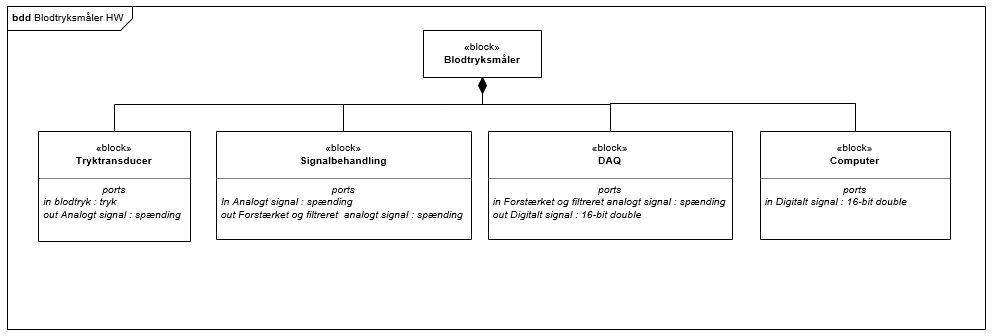
\includegraphics[width=1\textwidth]{Figurer/2}
	\caption{BDD}
	\label{fig:BDD}
\end{figure}

\begin{longtabu} to \linewidth{@{}l X[j]@{}}
	\textbf{Blok} &	\textbf{Beskrivelse} \\[-1ex]
	\midrule
	Blodtryksmåler & Det overordnede system, som indeholder Tryktransducer, Signalbehandling, DAQ og Computer.\\[-1ex]
	Tryktransducer & Registrerer en fysisk størrelse i form af en trykændring. Tryktransduceren har til opgave at transformere den fysiske størrelse til en elektrisk spænding, som viderebehandles gennem de resterne hardware blokke.  \\[-1ex]
	Signalbehandling & Består af to dele. En forstærkerdel og en filteringsdel. Det analoge signal fra tryktransduceren bliver via denne blok forstærket og filteret.\\[-1ex]
	DAQ & Konverterer det forstærkede og filterede analoge signal til et digitalt signal.\\[-1ex]
	Computer & Indeholder software til systemet, som er kodet i Visual Studio C\#. Softwaren kan blandt andet vise det digitale signal grafisk. Softwaren kan ligeledes kalibrere, nulpunktsjustere og gemme målinger samt aktivere og deaktiver filter.\\[-1ex]
	\caption{Beskrivelse af blokkene for systemet}
	\end{longtabu}
	
\subsection{IBD}
På figur 2.2 ses IBD for systemet. IBD viser, hvordan de forskellige hardware blokke interagerer med hinanden. IBD fortæller signalets behandling gennem systemet - altså hvordan signalet transformeres fra et målt fysisk tryk til et digitalt signal, som softwaren kan videre behandle og vise grafisk. 

\begin{figure}[H]
	\centering
	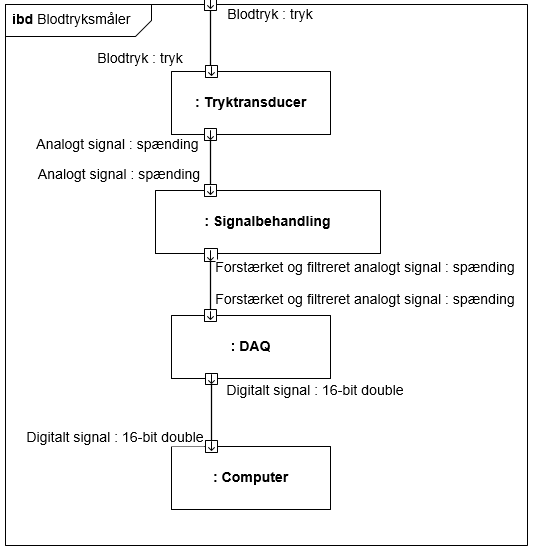
\includegraphics[width=0.8\textwidth]{Figurer/3}
	\caption{IBD}
	\label{fig:IBD}
\end{figure}

\section{Grænseflader}
Kommunikationsprotokol for hardware blokkene ses i tabel 2.3. Det er en beskrivelse og specifikation af hvilket indgang- og udgangssignal, de forskellige hardware blokke har. 
\\  \\
Tryktransducerens maximale output, $V_{max}$, bestemmes ud fra følgende ligning:

\begin{equation}
	V_{max} = P \cdot K \cdot V_{+}
\end{equation}

P = Tryk\\
K = sensitivitet\\
$V_{+}$ = indgangsspænding\\

For systemet er der valgt, at tryktransducerens målbare område skal ligge i intervallet 0-300 mmHg. Den maksimale udgangsspænding bliver derfor udtrykt fra det maksimale tryk på 300 mmHg, sensitiviteten på 5 $\mu$ og indgangsspændingen på 5 V. Indgangspændingen kommer reelt fra 9 V batterier, men der er valgt at indsætte en 5 V regulator, så man er sikker på, hvad indgangspændingen er, da batterier er ustabile.  


\begin{equation}
	V_{max} = 300 mmHg \cdot 5\mu V \cdot 5 V\\
\end{equation}
\begin{equation}
	V_{max} = 7,5 mV
\end{equation}


  

\begin{longtabu} to \linewidth{@{}l l l l X[j]@{}}
	\textbf{Grænseflade} & \textbf{Signal} & \textbf{Type} & \textbf{Format} & \textbf{Værdi} \\[-1ex]
	\midrule
	Tryktransducer & Blodtryk & in & Tryk & 0 - 300 mmHg \\[-1ex]
				& Analogt & out & Spænding & +/- 7,5 mV \\[-1ex]
	Signalbehandling  & Analogt & in & Spænding & +/- 7,5 mV \\[-1ex]
			 & Forstærket og filteret analogt & out & Spænding & +/- 5 V \\[-1ex]
	DAQ			& Forstærket og filteret analogt & in & Spænding & +/- 5 V \\[-1ex]	
				& Digitalt & out & 16-bit double & 0-5 V \\[-1ex]
	Computer	& Digitalt & in & 16-bit double &  0-5 V \\[-1ex]
	\caption{Kommunikationsprotokol}	
\end{longtabu}


\section{Hardware arkitektur}
Herunder er de krævede specifikationer for signalbehandlingsblokken beskrevet. Tryktransducerens beskrives ligeledes, da denne har indflydelse for forstærkerblokkens specifikationer. 

\subsubsection{Tryktransducer}
Tryktransduceren skal omsætte det fysiske tryk til en elektrisk spænding. Tryktransduceren har en meget høj common mode rejection samt en høj sensitivitet på 5 $\mu$V/V/mmHg +/- 1 \% \footnote{Se datablad for tryktransduceren i bilag} , da de forventede trykændringer er små. Enheden for sensitiviteten angiver hvor mange $\mu$V output, der kommer fra tryktransduceren pr. antal V i tryktransducerens eksitationsspænding pr. mmHg.

\subsubsection{Forstærkerblok}
Forstærkerblokken sørger for, at det meget svage spændingssignal fra tryktransduceren bliver forstærket op til en spænding, der ligger indenfor det måleinterval, der svarer til DAQ'en, som er valgt til +/- 5 V.
 
\subsubsection{Filterblok}
Filterets formål er at frasortere signalets frekvenser, der er højere end 50 Hz, da disse ikke har nogen relevans for blodtryksignalet. Dette skal realiseres ved et andenordens lavpasfilter. 
 
\subsection{BDD}
På figur 2.3 ses BDD for signalbehandlingsblokken, hvor forstærkerblokkens og filterblokkens indgang- og udgangsporte er vist.  
\begin{figure}[H]
	\centering
	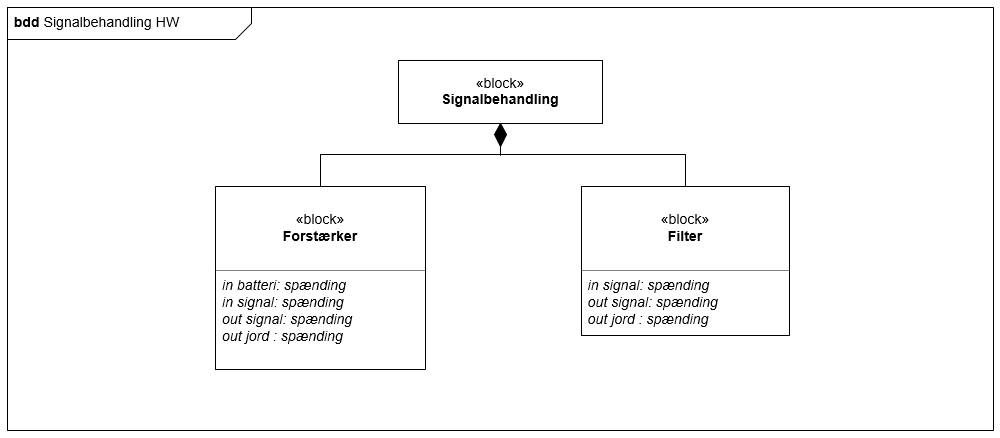
\includegraphics[width=1\textwidth]{Figurer/4}
	\caption{BDD for Signalbehandling HW}
	\label{fig:BDDhw-diagram}
\end{figure}

\subsection{IBD}
På figur 2.4 ses IBD for signalbehandlingsblokken. IBD viser, hvordan forstærkerblokken og filterblokken interagerer med hinanden. 

\begin{figure}[H]
	\centering
	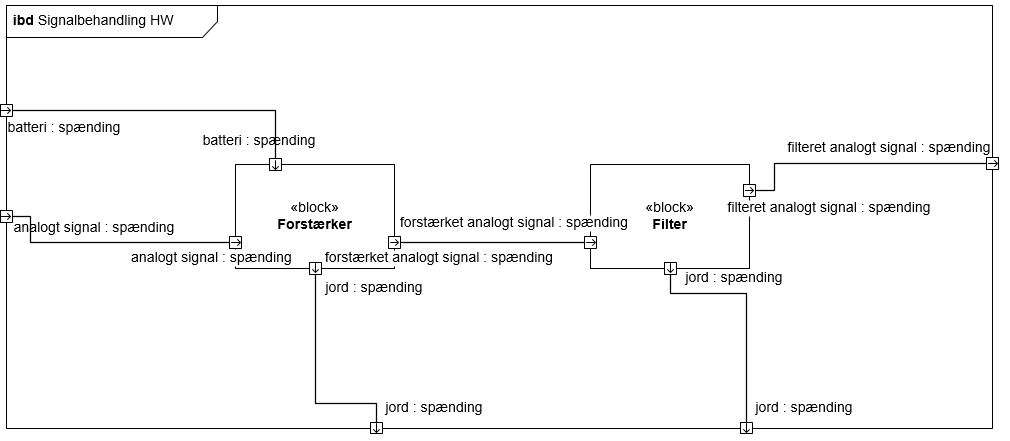
\includegraphics[width=1\textwidth]{Figurer/5}
	\caption{IBD for Signalbehandling HW}
	\label{fig:IBDhw-diagram}
\end{figure}

\subsection{Grænseflader}

\begin{longtabu} to \linewidth{@{}l l l l X[j]@{}}
	\textbf{Grænseflade} & \textbf{Signal} & \textbf{Type} & \textbf{Format} & \textbf{Værdi} \\[-1ex]
	\midrule
	Forstærker & Batteri & in & Spænding & +/- 9 V \\[-1ex]
			   & Analogt & in & Spænding & +/- 7,5 mV \\[-1ex]
			   & Jord	 & out & Spænding & 0 V \\[-1ex]
			   & Forstærket analogt & out & Spænding & +/- 5 V \\[-1ex]
	Filter	   & Forstærket analogt & in & Spænding & +/- 5 V\\[-1ex]
			   & Jord	 & out & Spænding & 0 V\\[-1ex]
			   & Filteret analogt & out & Spænding & +/- 5 V\\[-1ex]
	\caption{Kommunikationsprotokol for Instrumenteringsforstærke}	
\end{longtabu}


 \subsection{Forstærkerblok}
 \subsubsection{Specifikationer}
 \begin{itemize}
 	\item Forstærkningen, Gain, skal forstærke den maksimale inputsspænding, så outputtet bliver 5 V
 	\begin{equation}
 		Gain \cdot V_{in} = V_{out}
 	\end{equation}
 	
 	$V_{out}$ og $V_{in}$ er kendt, så Gain isoleres
 	
 	\begin{equation}
 		Gain = \frac{V_{out}}{V_{in}} \\ \Longrightarrow \\
 		Gain = \frac{5000 mV}{7,5 mV}\\ \Longrightarrow \\
 		Gain = 666,667
 	\end{equation}
 	
 	
 	
 	\item Indgangspænding: +/- 7,5 mV
 	\item Eksitationsspænding: +/- 9 V
 	\item Outputspænding: +/- 5 V
 	\item Minimum en båndbredde på 50 Hz
 	\item Uendelig indgangsimpedans i teorien
 \end{itemize}


 \subsection{Filterblok}
 \subsubsection{Specifikationer}
 \begin{itemize}
 	\item Andenordens lavpasfilter
 	\item Cutofffrekvens ved 50 Hz
 	\item Unity gain (ingen forstærkning)
 	\item -40 dB ved 500 Hz
 	\item Uendelig indgangsimpedans i teorien
 	\item Indgangsspænding +/- 5 V
 	\item Eksitationsspænding +/- 9 V
 \end{itemize}
 

\section{Software arkitektur}

\subsection{Domænemodel}
Domænemodellen er skabt på baggrund af de seks Use Cases og fungerer som et middel til at skabe et samlet overblik over systemet. Gennem navneordsanalyse er de konceptuelle klasser fundet. I modellen beskrives, hvordan de konceptuelle klasser og aktører interagerer med hinanden. Controlleren er ikke en konceptuel klasse, men det er den, der sørger for at systemet fungerer optimalt, og udfører kommandoer.

\begin{figure}[H]
	\centering
	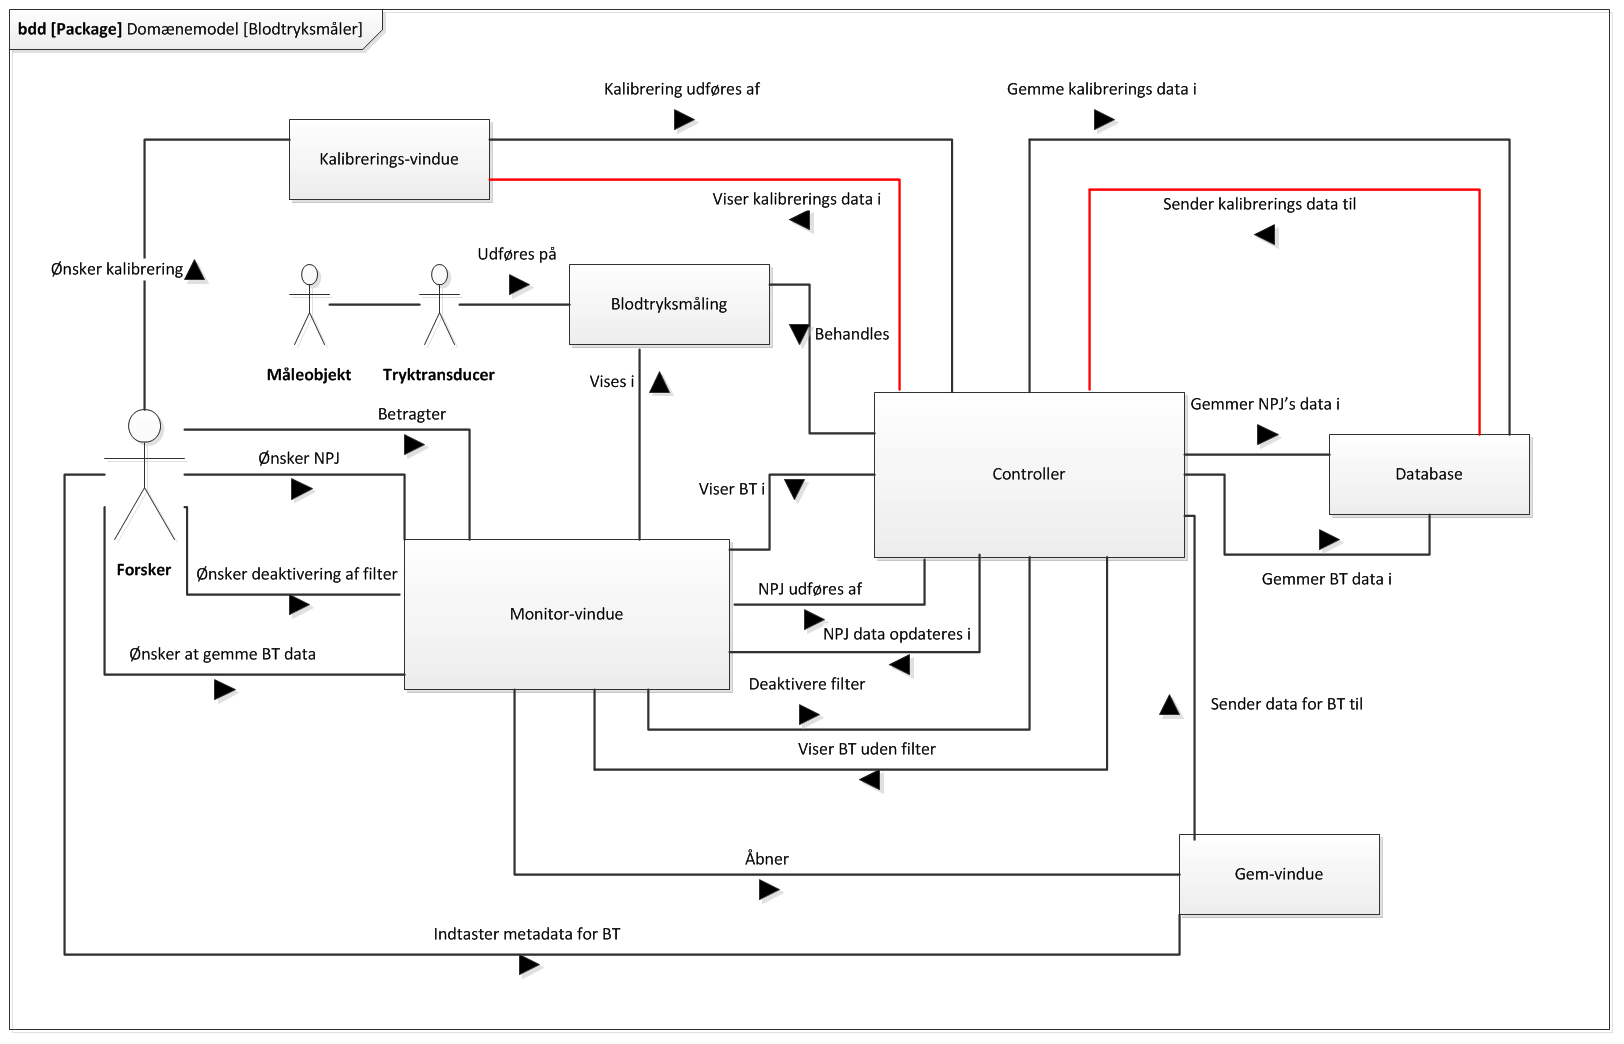
\includegraphics[width=1 \textwidth]{Figurer/Snip20151104_30}
	\caption{Domænemodel for blodtryksmålersystemet}
\end{figure}

NPJ = nulpunktsjustering\\
BT = blodtryksmåling
\\ \\
I domænemodellen ses to røde streger, som har hver deres kommando – ”kalibrerings data bliver sendt fra database” og ”vises i kalibrerings-vinduet”.Årsagen til at stregerne er røde, er, at hver af de to handlinger udelukkende forekommer ved start/genstart af programmet.

\subsection{Applikationsmodel}

\subsubsection{Sekvensdiagram}
Sekvensdiagrammerne beskriver step-by-step, via metoder, forløbet i de forskellige Use Cases. Der er lavet et sekvensdiagram for hver Use Case, for at gøre systemet mere overskueligt. Et sekvensdiagram består af boundary-klasserne og domain-klasserne fra domænemodellen, samt en controller-klasse, med navn efter den specifikke Use Case.

\begin{figure}[H]
	\centering
	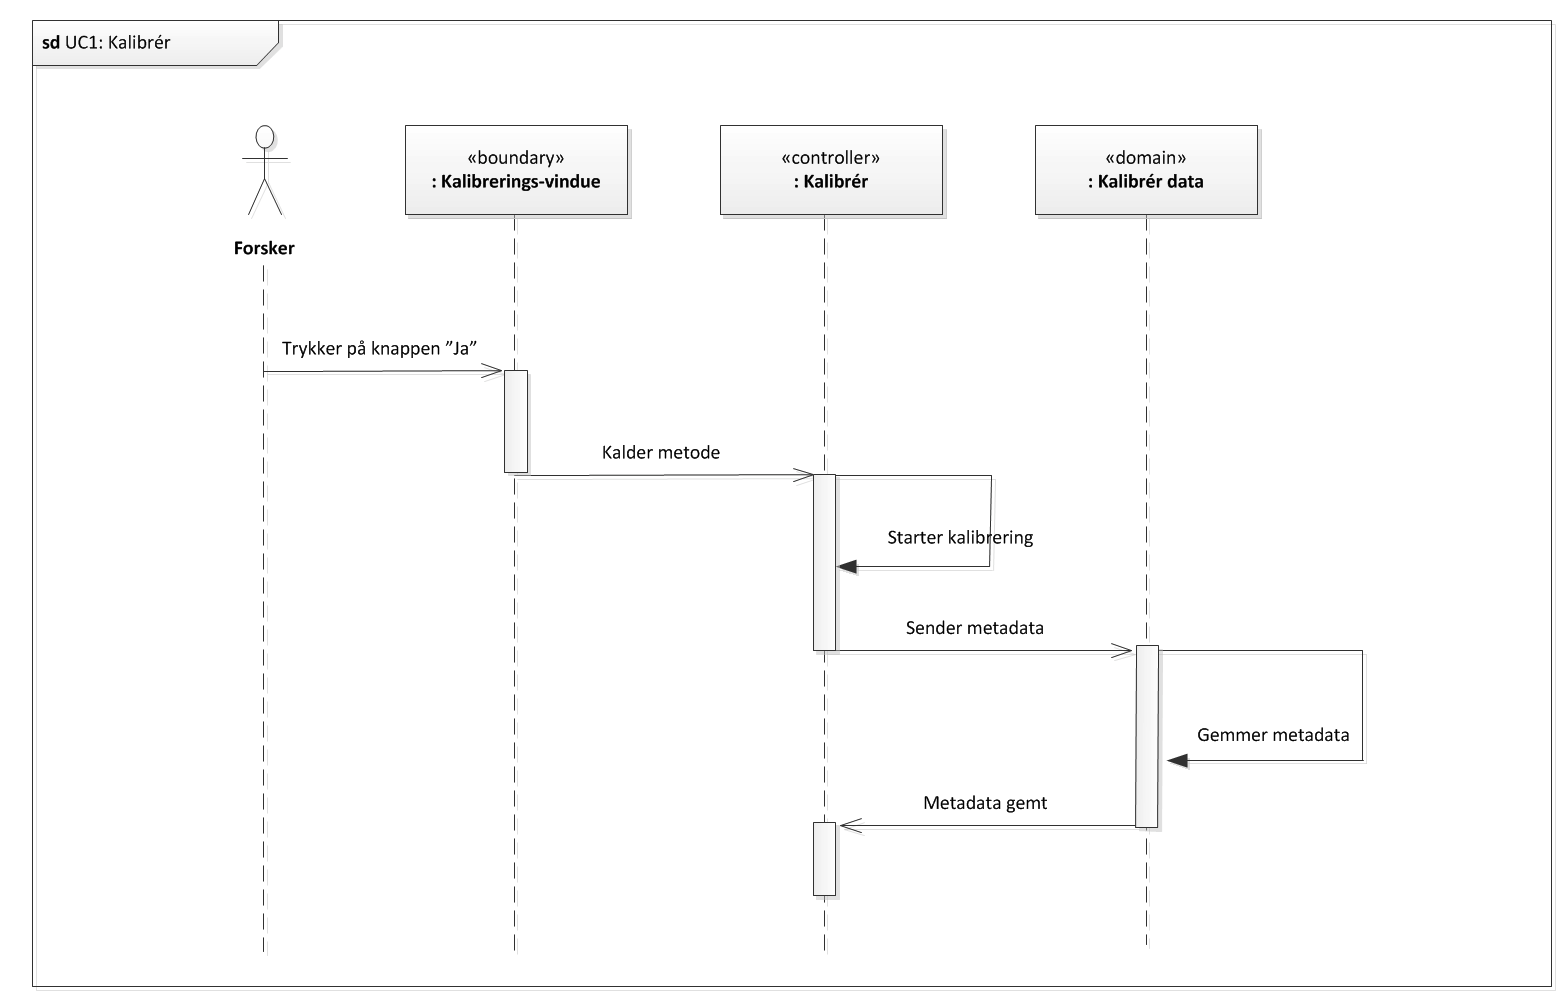
\includegraphics[width=1\textwidth]{Figurer/Snip20151104_31}
	\caption{Sekvensdiagram for UC1}
\end{figure}

Forsker interagerer med Monitorvindue. Kalibreringsmetoden bliver kaldt, når Forsker trykker på knappen ”Ja”. Derefter igangsættes kalibreringen og kalibrerings tidspunkt og værdi sendes og gemmes i databasen. 

\begin{figure}[H]
	\centering
	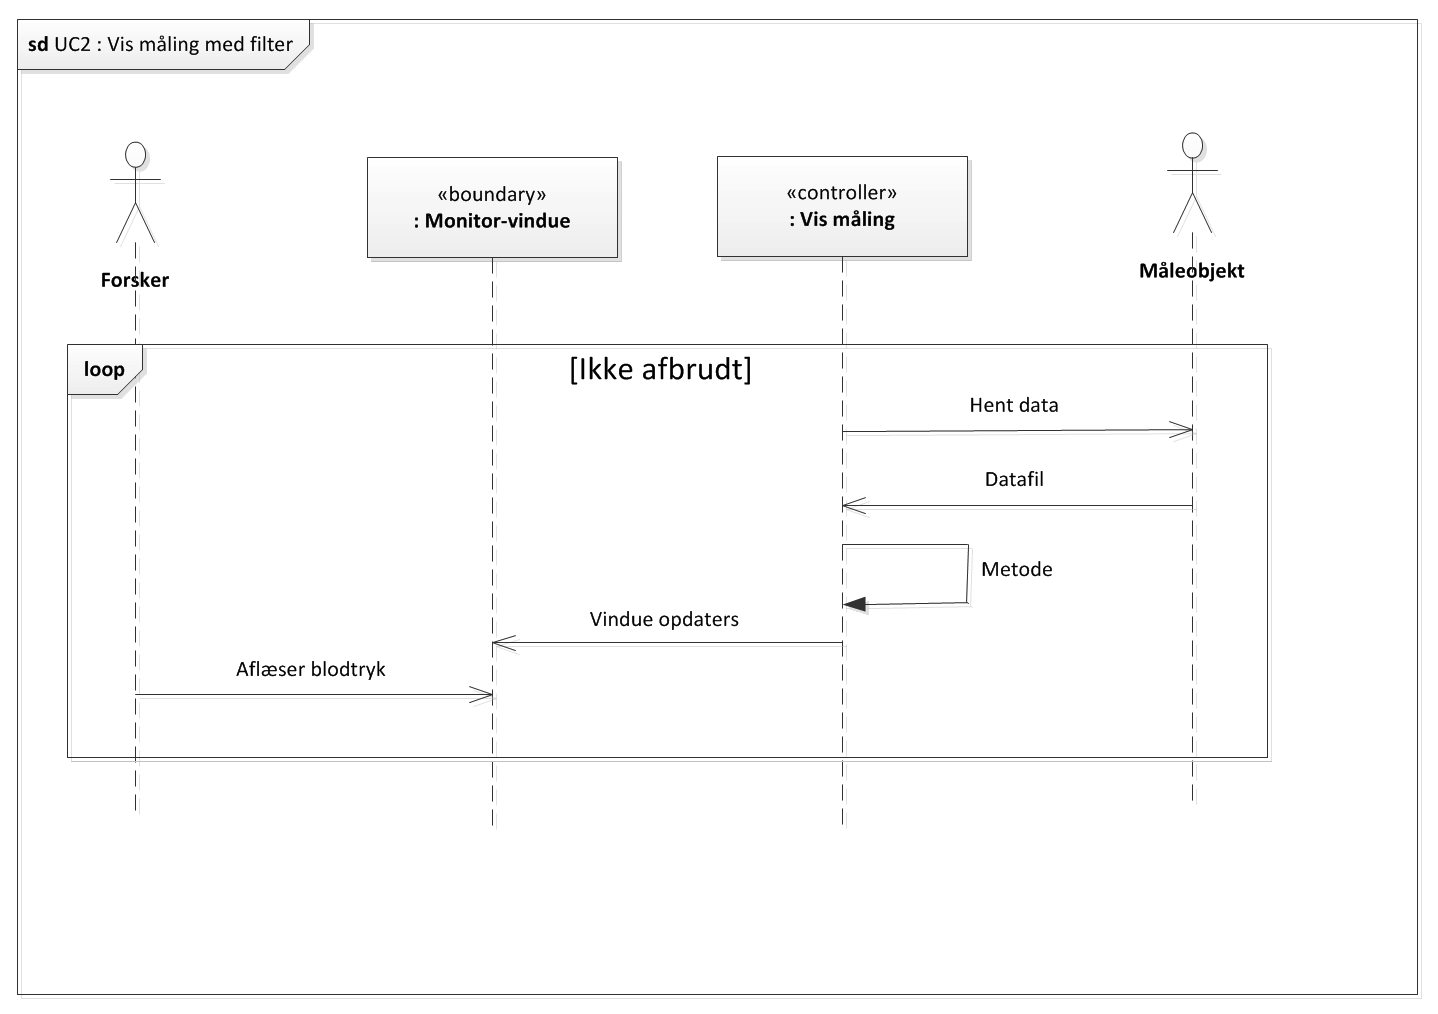
\includegraphics[width=1\textwidth]{Figurer/Snip20151104_32}
	\caption{Sekvensdiagram for UC2}
\end{figure}

Controller henter data fra Tryktransducer, som henter data i form af tryk fra måleobjekt. Datafilerne sendes fra Måleobjekt via Tryktransducer tilbage til Controller, der kalder metoden. Monitorvindue opdateres, og herefter kan Forsker aflæse blodtryk. 

\begin{figure}[H]
	\centering
	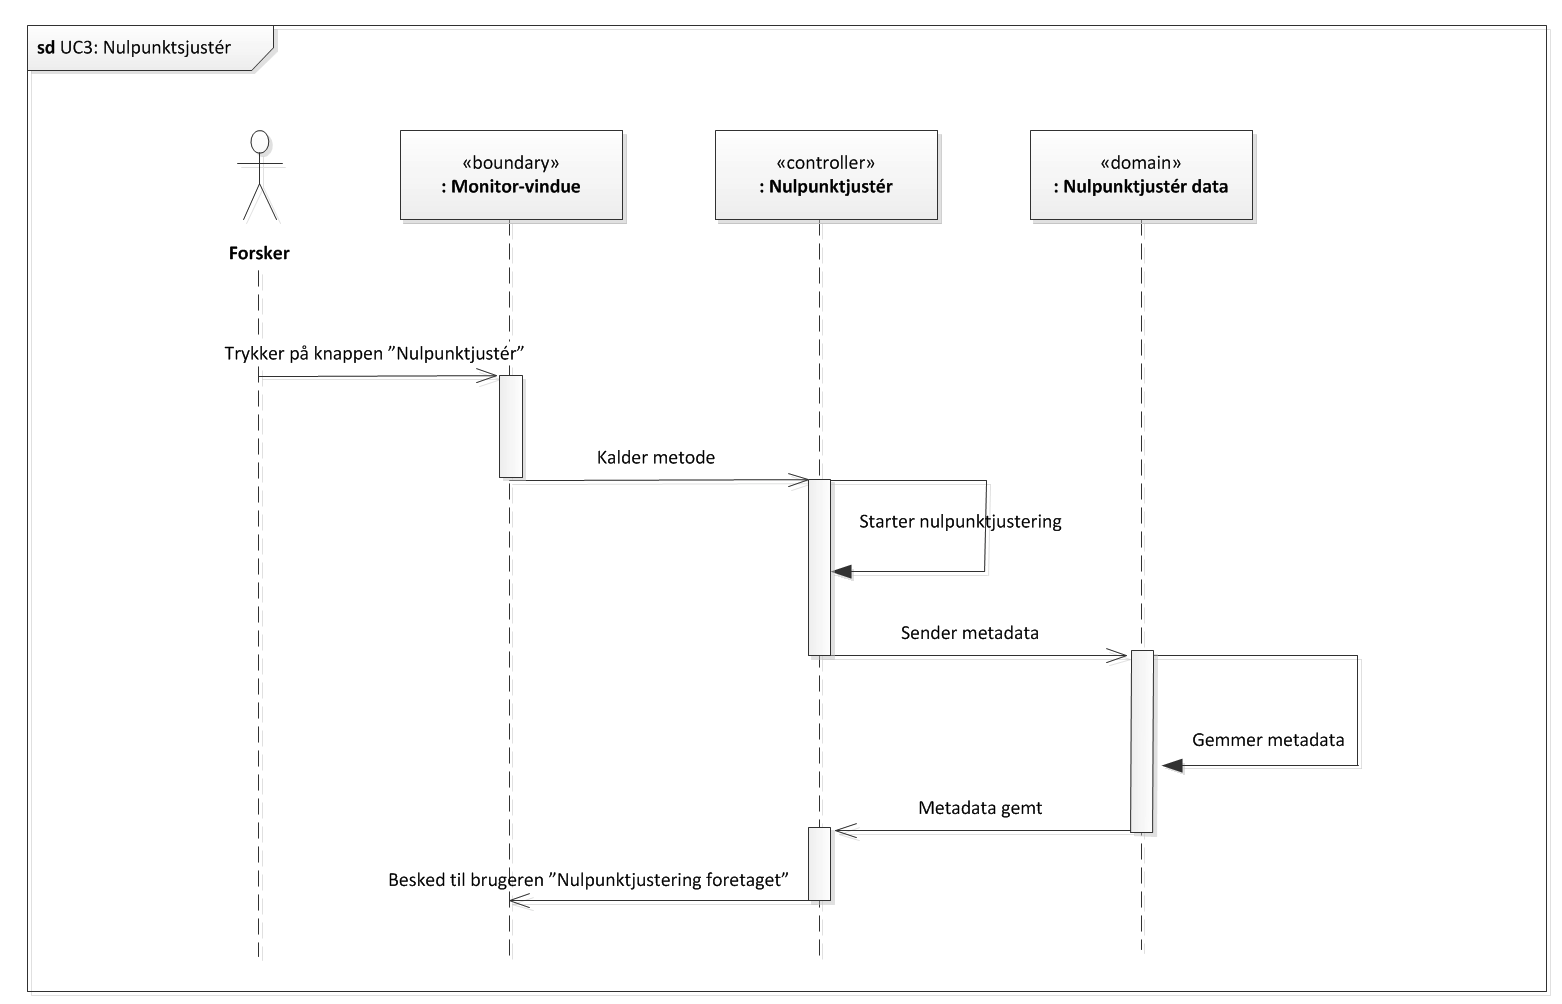
\includegraphics[width=1\textwidth]{Figurer/Snip20151104_33}
	\caption{Sekvensdiagram for UC3}
\end{figure}

Forsker interagerer med Monitorvindue ved at trykke på knappen ”Nulpunktsjustér”. Derefter kaldes metoden, og nulpunktsjusteringen startes. Tidspunktet og værdien for nulpunktjusteringen sendes og gemmes i databasn, hvorefter Forsker får besked om, at nulpunktsjusteringen er foretaget. 

\begin{figure}[H]
	\centering
	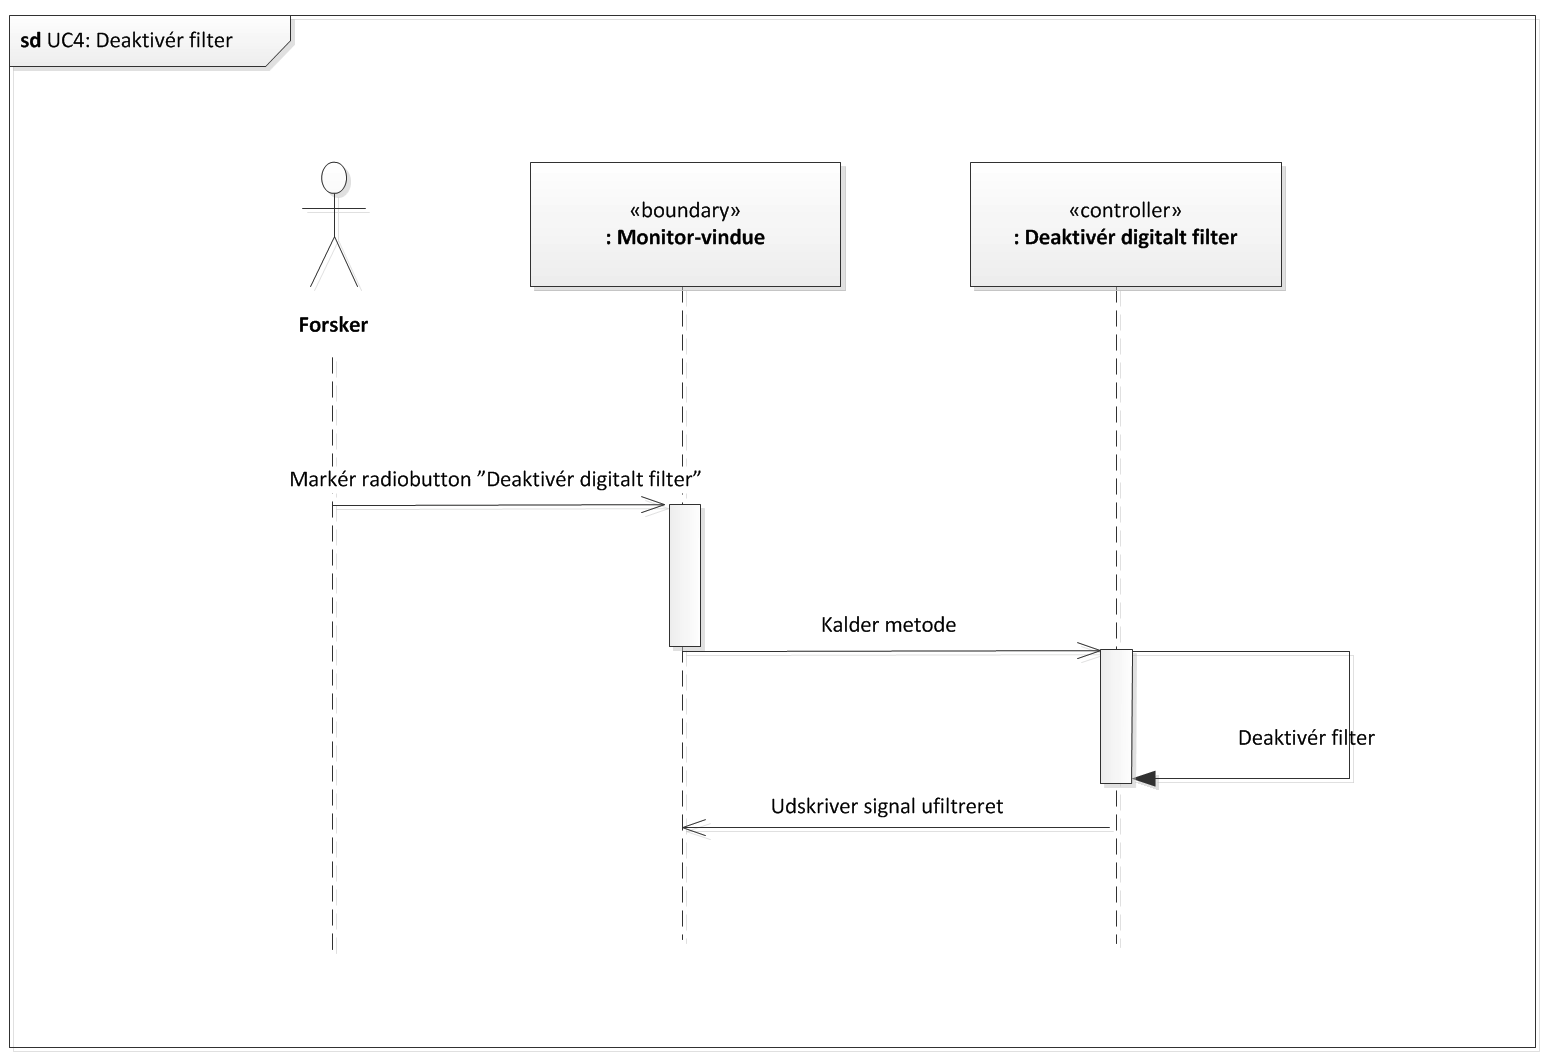
\includegraphics[width=1\textwidth]{Figurer/Snip20151104_34}
	\caption{Sekvensdiagram for UC4}
\end{figure}

Forsker interagerer med Monitorvindue ved at markere i radiobutton ”Deaktivér digitalt filter”. Derefter kaldes metoden, og filteret deaktiveres, hvorefter signalet bliver udskrevet ufiltreret.

\begin{figure}[H]
	\centering
	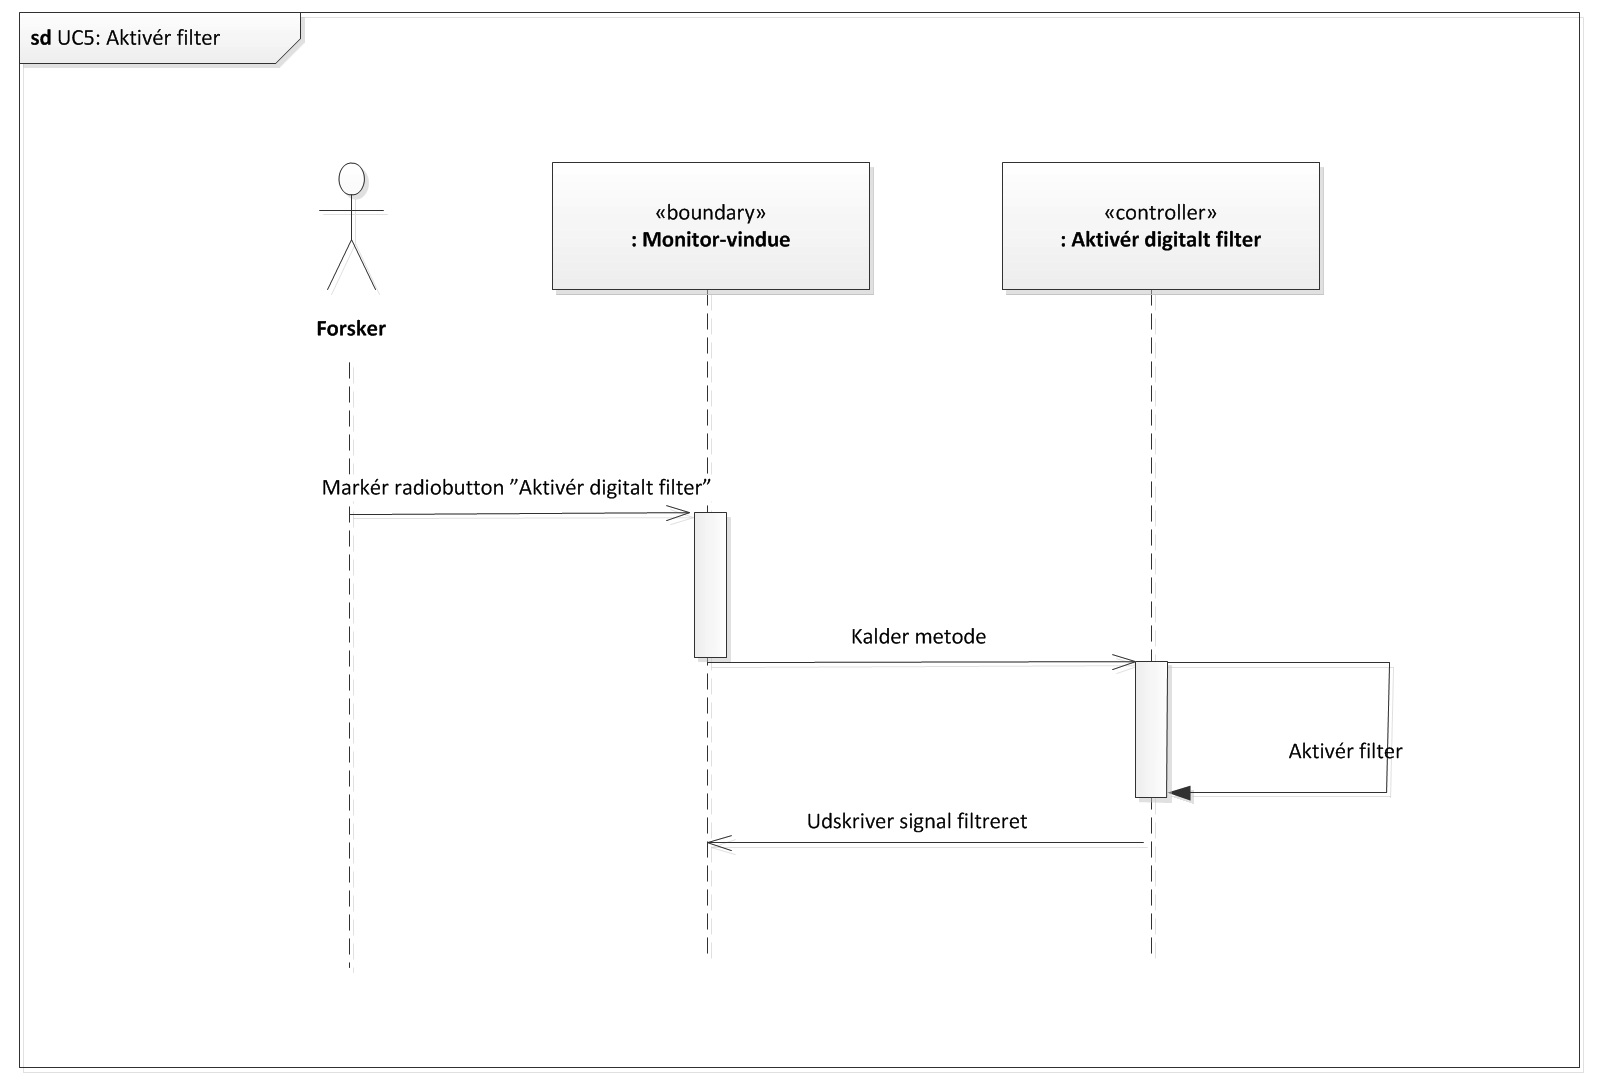
\includegraphics[width=1\textwidth]{Figurer/Snip20151104_35}
	\caption{Sekvensdiagram for UC5}
\end{figure}

Forsker interagerer med Monitorvindue ved at markere i radiobutton ”Aktivér digitalt filter”. Derefter kaldes metoden, og filteret aktiveres, hvorefter signalet bliver udskrevet filtreret.

\begin{figure}[H]
	\centering
	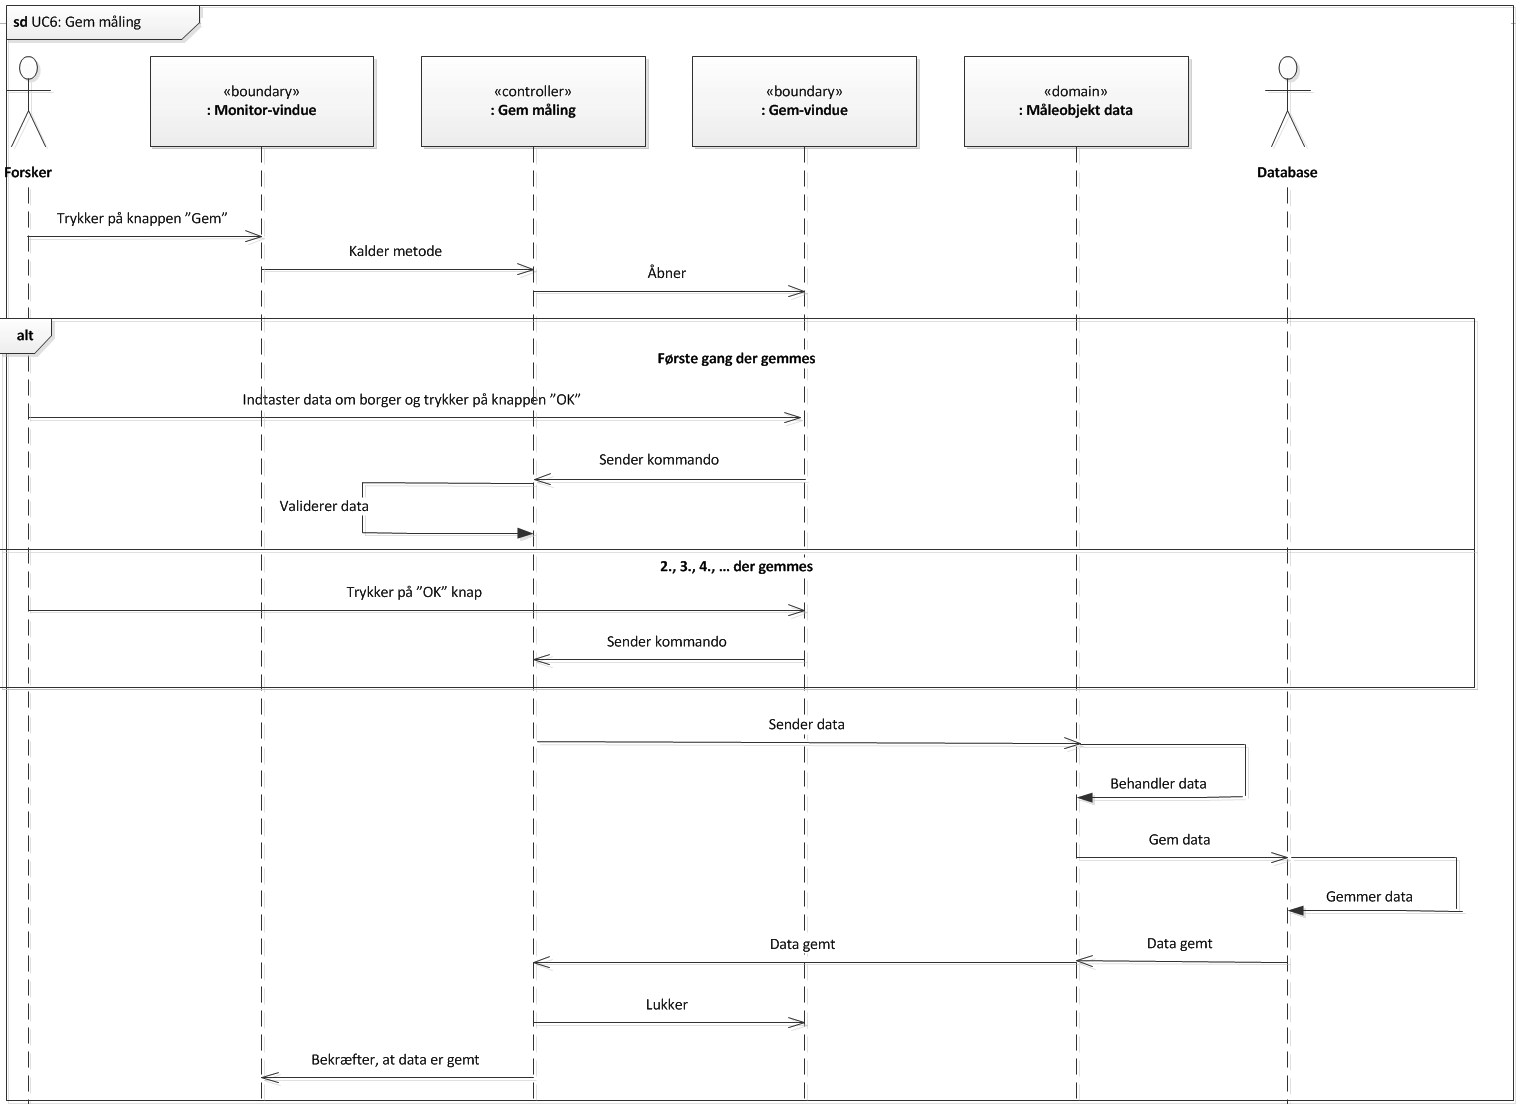
\includegraphics[width=1\textwidth]{Figurer/Snip20151104_36}
	\caption{Sekvensdiagram for UC6}
\end{figure}

Forsker interagerer med Monitorvindue ved at trykke på knappen ”Gem”. Derefter kaldes metoden og Gem-vinduet åbnes. Første gang Forsker ønsker at gemme, indtastes data om målingen og der trykkes på knappen ”OK”. Kommando sendes og data gemmes. De efterfølgende gange, der ønskes at gemme, er data udfyldt fra første gang, og der trykkes blot på ”OK”, hvorefter kommandoen sendes. Data gemmes og Gem vinduet lukkes. Controller bekræfter til Monitorvindue, at data er gemt.

\subsubsection{Opdateret klassediagram}
De opdateret klassediagrammer indeholder metoderne fra de dertilhørende  sekvensdiagrammer - dette giver et overblik over, hvilke metoder de forskellige klasser består af.

\begin{figure}[H]
	\centering
	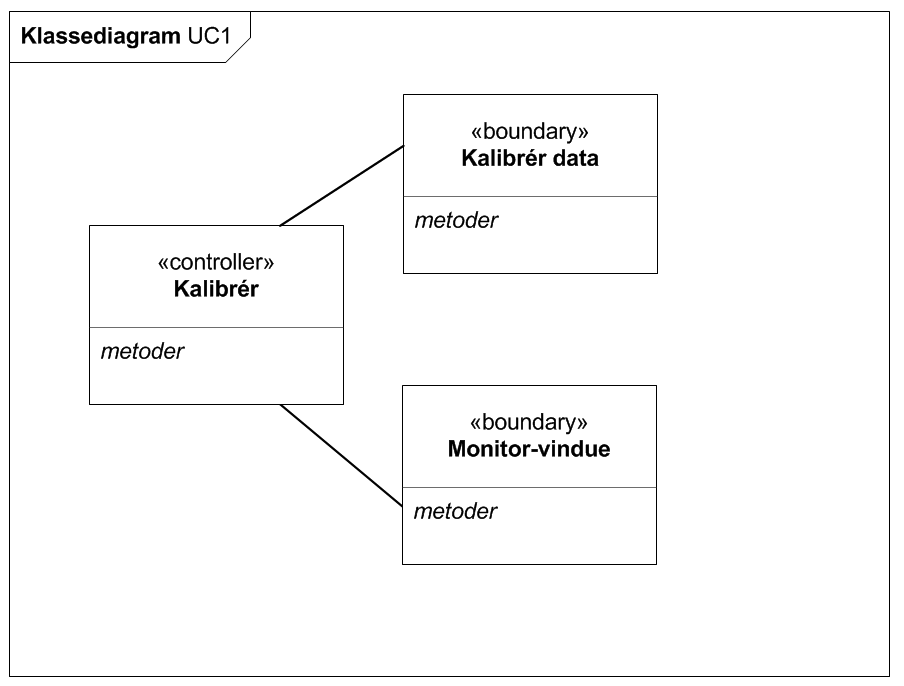
\includegraphics[width=1\textwidth]{Figurer/Snip20151104_37}
	\caption{Klassediagram for UC1}
\end{figure}
 

\begin{figure}[H]
	\centering
	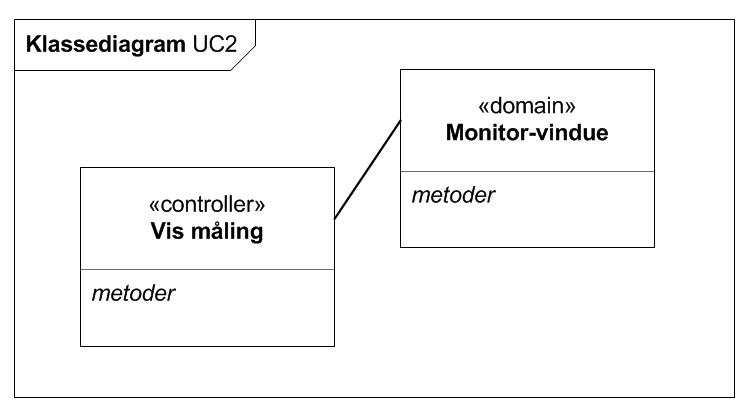
\includegraphics[width=1\textwidth]{Figurer/Snip20151104_38}
	\caption{Klassediagram for UC2}
\end{figure}

\begin{figure}[H]
	\centering
	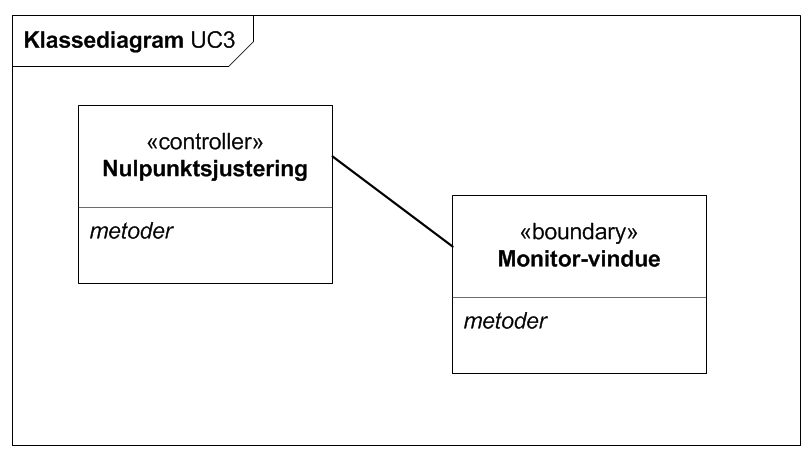
\includegraphics[width=1\textwidth]{Figurer/Snip20151104_39}
	\caption{Klassediagram for UC3}
\end{figure}

\begin{figure}[H]
	\centering
	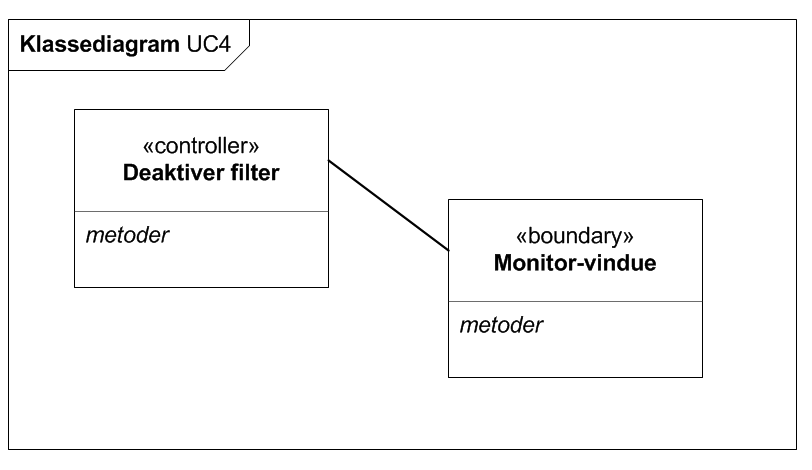
\includegraphics[width=1\textwidth]{Figurer/Snip20151104_40}
	\caption{Klassediagram for UC4}
\end{figure}

\begin{figure}[H]
	\centering
	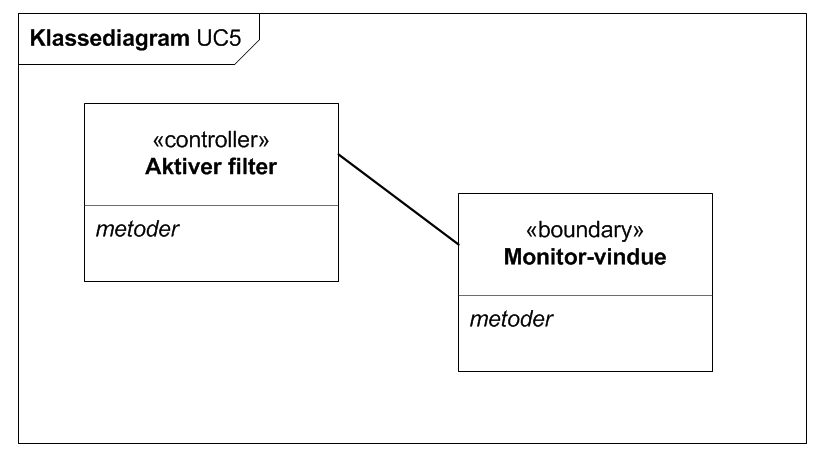
\includegraphics[width=1\textwidth]{Figurer/Snip20151104_41}
	\caption{Klassediagram for UC5}
\end{figure}

\begin{figure}[H]
	\centering
	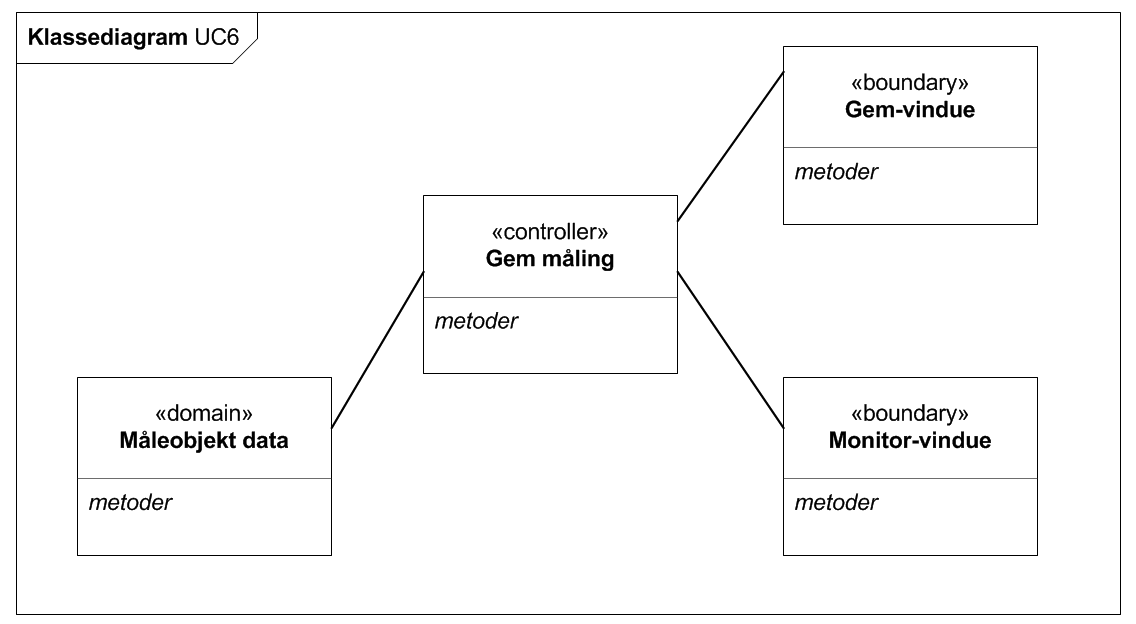
\includegraphics[width=1\textwidth]{Figurer/Snip20151104_42}
	\caption{Klassediagram for UC6}
\end{figure}












